\chapter{Introduction}

The scheduling of conventional thermal power plants is crucial with the rise of renewable energies.
The Unit Commitment Problem (UCP) tackles this problem~\cite{Banos2011}.
Also, it can be used with wind energy and thermal power plants to minimize the cost of incorrect weather predictions.
These approaches are also called risk-based because they model the risk of the weather predictions being wrong~\cite{Chen2008, Abujarad2017}.

The number of deployed smart meters in the European Union was 99 million in 2018.
A study by the European Commission projected the number to reach 123 million by 2020~\cite{Vlachogiannis2019}.
With the increasing number of smart meters, the amount of information about energy consumption is growing.
The data is available with a time resolution that was not yet possible.
Due to this large amount of data, predicting future power consumption is possible on a house-to-house basis.
That allows for a much better overall prediction of the power consumption of towns or cities~\cite{Aiello2016, Basu2013}.
It presents the possibility to schedule thermal power plants much more precisely and with a higher time resolution.

In the future, communities with many private renewable energy sources might rely on distributed energy generation.
Distributed energy generation means that the energy produced by a consumer through their renewable energy sources gets added to the grid if the consumer is currently not using this energy~\cite{Aiello2016}.
Additionally, electric vehicles can be used as energy sources when plugged into a charger~\cite{Zhang2016}.
The addition of these energy sources gives additional degrees of freedom for energy procurement.

Figure \ref{figure:problem.sketch} is a sketch of the problem that the work considers.
It shows a town with offices and houses, as well as charging stations for electric vehicles.
There are $4$ power plants around the town that are all connected to it.

Optimizing the UCP takes a lot of time for large inputs.
Large inputs here means one of two things or both:
\begin{enumerate*}[label=(\roman*)]
  \item More units, i.e., power plants or
  \item A longer timeframe, over which to schedule the units.
\end{enumerate*}
UCPs are optimization problems and thus, most of the time formulated as Mixed-integer Non-linear Problems~\cite{Baldick1995}.
Precisely optimizing these problems is NP-complete~\cite{Li2005, Bienstock1996}.
The energy industry needs faster algorithms for large inputs to deal with the increasing amount of information.
These algorithms also have to be precise.

Quantum computing promises optimization algorithms with improved time complexity~\cite{Portnov2000, Ahuja1999, Gilliam2019, Ajagekar2020, Shaydulin2019}.
There are two types of quantum processors.
One of which is designed for optimizations and the other which is a more general quantum processor.

Today's quantum computers are described as Noisy Intermediate-Scale Quantum (NISQ) technology.
That is because the hardware is sensitive to noise and thus not able to run long computations.
Also, there are not many qubits in the latest quantum computers (intermediate-scale)~\cite{Leymann2020}.
That is why one can't run most quantum algorithms for practical problems.
Either there are not enough qubits to represent the variables, or the result is too noisy.
One alternative that still can give a speed-up for some problems are hybrid classical-quantum algorithms.
Such algorithms solve the problem at hand with classical computers and use quantum computers to speed up specific parts that a NISQ quantum computer can compute~\cite{Ajagekar2020, Shaydulin2019}.

This work explores the application of purely quantum and hybrid classical-quantum algorithms to the UCP.
It compares their performance in regards to computation time and accuracy of the result.
The goal is to find an algorithm that can accurately solve large UCPs faster than the current classical algorithms.

\begin{figure}[!ht]
  \centering
  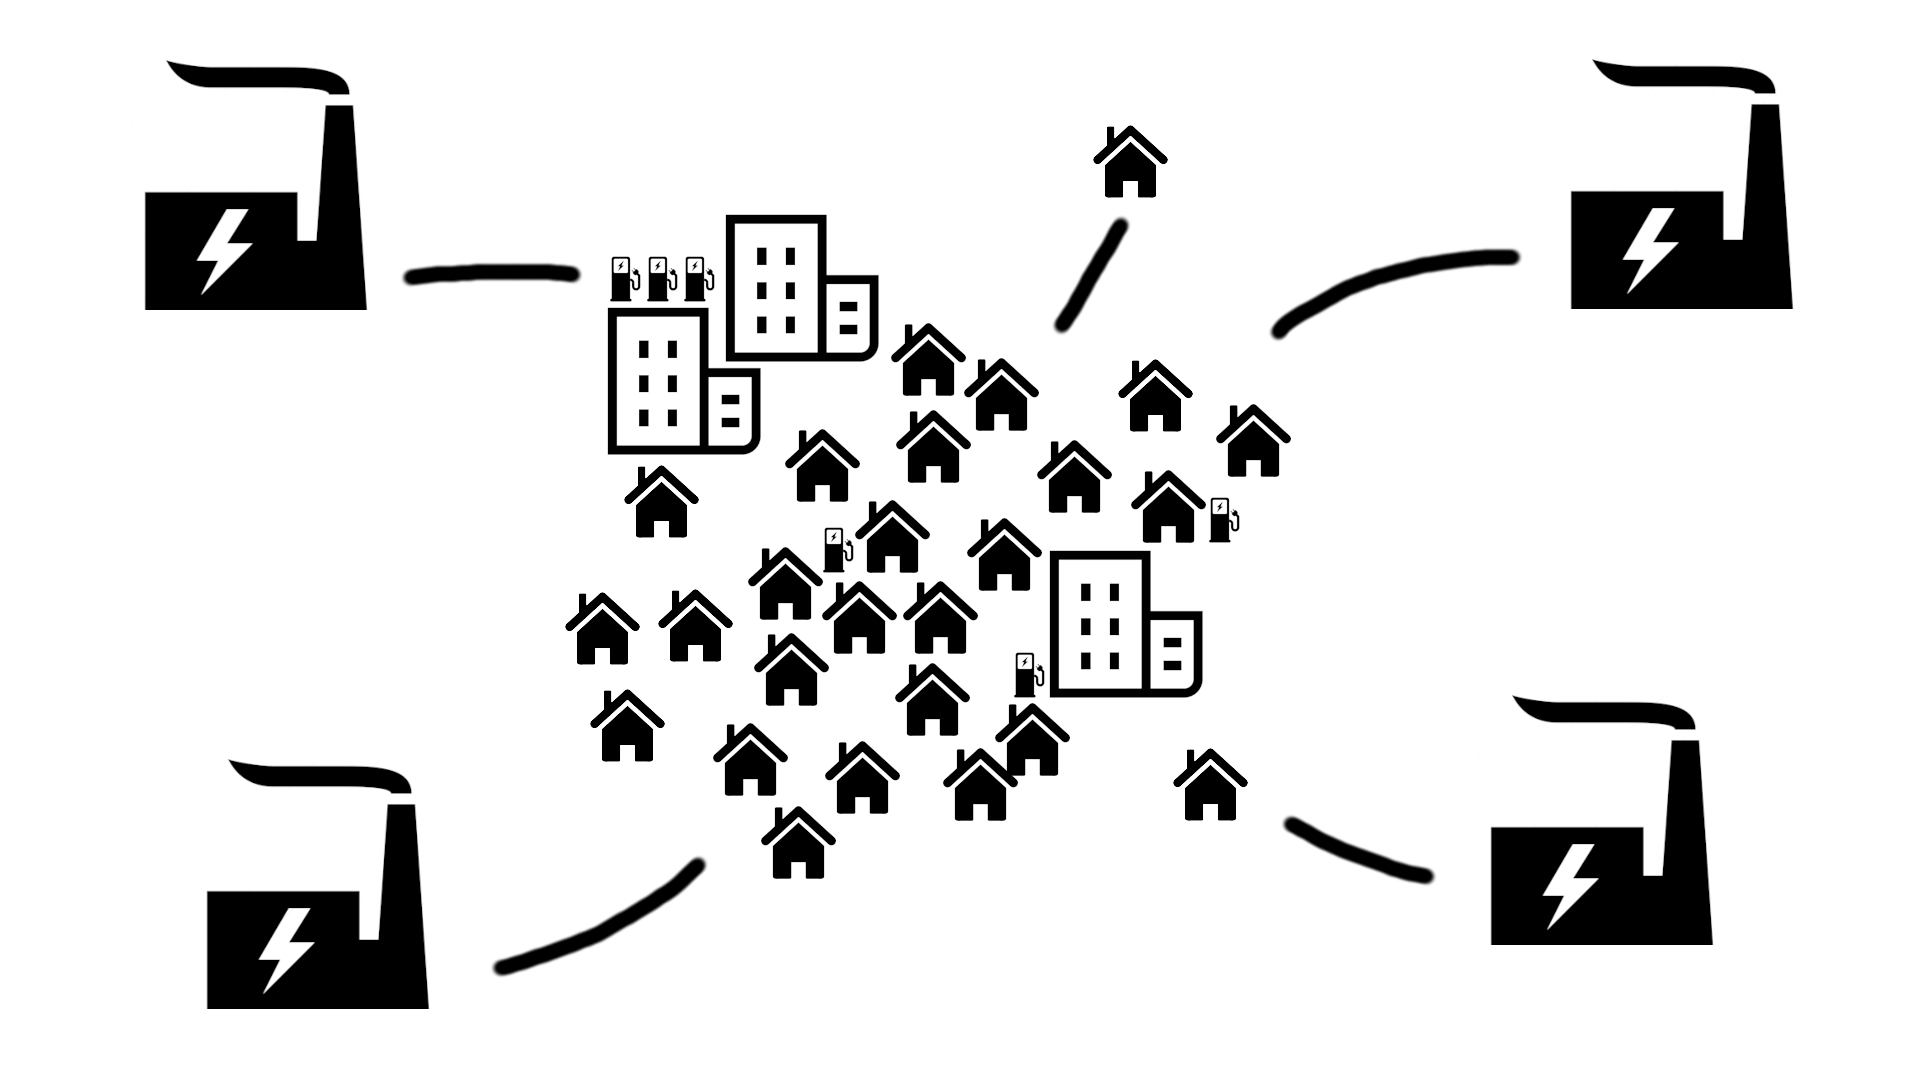
\includegraphics[width=\textwidth]{01_Intro/problem_sketch.png}
  \caption{Sketch of Unit Commitment Problem}
  \label{figure:problem.sketch}
\end{figure}
